% =========================================================================== %

\begin{frame}[t,plain]
\titlepage
\end{frame}

% =========================================================================== %

\begin{frame}{Drinking Fountains}
%
\begin{columns}
\column{.5\linewidth}
\begin{center}
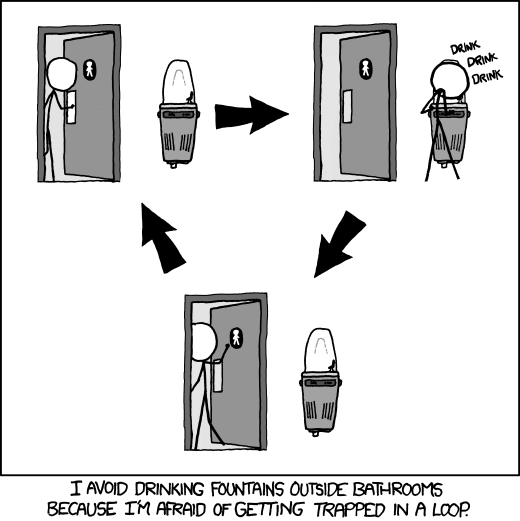
\includegraphics[width=.9\linewidth]{./gfx/08-xkcd-drinking-fountains}\\
\end{center}
%
\column{.4\linewidth}
\small
	\emph{\enquote{I've always wondered whether you could drink slowly enough, and eliminate fast enough, that you just sort of peed continuously.
		  But I'm afraid to try because I worry someone might call while I'm doing it and ask what I'm up to, and I won't be able to think of a lie.}}

	\vspace{6pt}
	\url{https://xkcd.com/986/}
\end{columns}
%
\end{frame}

% =========================================================================== %

\begin{frame}{Scope For Today}
%
\begin{itemize}
\item \inPy{for}-loops under the hood
	\begin{itemize}
	\item Iterables and Iterators
	\item The command \inPy{yield}
	\item Generator expressions
	\item Iterator invalidation
	\end{itemize}
\item Functional Programming and Lazy Evaluation
	\begin{itemize}
	\item \inPy{map} and \inPy{filter}
	\item Short Circuiting
	\end{itemize}
\item The module \texttt{itertools}
	\begin{itemize}
	\item \texttt{count}, \texttt{cycle} and \texttt{repeat}
	\item \texttt{starmap}, \texttt{filterfalse}, \texttt{dropwhile} and \texttt{takewhile}
	\item \texttt{functools.reduce} and \texttt{itertools.accumulate}
	\item \texttt{product}, \texttt{permutations}, \texttt{combinations}, \texttt{combinations\_with\_replacement}
	\end{itemize}
\end{itemize}
%
\end{frame}

% =========================================================================== %

\begin{frame}[fragile]{Iterators and Iterables: Definition}
%
\begin{columns}
\column{.6\linewidth}
\begin{defbox}[Iterable]
An iterable is any instance of a class that provides an \inPy{__iter__} method which returns an iterator.
\end{defbox}
%
\begin{defbox}[Iterator]
An iterator is any instance of a class that provides a \inPy{__next__} method which either returns a value or raises \inPy{StopIteration}.
\end{defbox}
%
\column{.3\linewidth}

\includegraphics[width=\linewidth]{./gfx/08-geek}
\emph{So, everything's clear, right?}

\vspace{6pt}
\begin{flushright}
\tiny
\href{https://www.shutterstock.com/image-photo/beautiful-geek-woman-holding-digital-tablet-421481161}{Image Source: Shutterstock}
\end{flushright}
\end{columns}
%
\end{frame}

% =========================================================================== %

\begin{frame}[fragile]{Iterators and Iterables: \emph{Useful} Definitions}
%
\begin{defbox}[Iterable]
An iterable is any object that we can loop over in a \inPy{for} loop. Examples include \inPy{list}s, \inPy{dict}s and file descriptors.
\end{defbox}
%
\begin{defbox}[Iterator]
An iterator is a (usually temporary) book keeping device that provides the means to find the next object or detect the end of the iterable when looping over it.
They are automatically generated in \inPy{for} loops.
\end{defbox}
%
\end{frame}

% =========================================================================== %

\begin{frame}[fragile]{In a Nutshell -- \inPy{for}-Loops Under the Hood}
%
\begin{itemize}
\item When running a \inPy{for}-loop, an iterator is automatically generated
\item This iterator is generated by the iterable
	\begin{itemize}
	\item \inPy{for} implies a call to the iterables \inPy{__iter__} method
	\item \inPy{__iter__} returns the iterator
	\item The presence of an \inPy{__iter__} method solely defines an iterable
	\end{itemize}
\item The iterator
	\begin{itemize}
	\item \enquote{knows} how to find the next object within the iterable
	\item reveals the next item via its \inPy{__next__} method
	\item raises \inPy{StopIteration} when the last element has been reached
	\item Each go through the loop calls \inPy{__next__} once
	\end{itemize}
\end{itemize}
%
\begin{hintbox}[Mixed Character]
\footnotesize
Often, an iterator also has an \inPy{__iter__} method, \ie is an iterable itself. It usually just returns \inPy{self}.
\end{hintbox}
%
\end{frame}

% =========================================================================== %

\begin{frame}[fragile]
%
\begin{codebox}[The Code You Write]
\begin{minted}[fontsize=\footnotesize]{python3}
for element in iterable:
    ...
\end{minted}
\end{codebox}
%
\begin{codebox}[What Python Actually Does]
\begin{minted}[fontsize=\footnotesize]{python3}
iterator = iter(iterable)
while True:
    try:
        element = next(iterator)
        ...
    except StopIteration:
        break
\end{minted}
\end{codebox}
%
\begin{hintbox}[Magic Methods]
\footnotesize
\inPy{iter(iterable)} calls \inPy{iterable.__iter__}.\\
\inPy{next(iterator)} calls \inPy{iterator.__next__}.
\end{hintbox}
%
\end{frame}

% =========================================================================== %

\begin{frame}{So What's It Good For?}
%
\begin{itemize}
\item We can make our own class instances iterable
	\begin{itemize}
	\item E.\;g.: advanced data structures like trees
	\item E.\;g.: objects that only generate the next number in line without storing the entire sequence
	\item[\Thus] Possibly infinite sequences
	\end{itemize}
\item Standardized Interface makes own iterables compatible with a lot of Python-builtins and third-party libraries
	\begin{itemize}
	\item E.\;g. \inPy{min}, \inPy{max}, \inPy{sum}
	\item E.\;g. \inPy{list}, \inPy{tuple}
	\item E.\;g. \texttt{matplotlib.pyplot.plot} and \texttt{numpy.array}
	\item Et cetera
	\end{itemize}
\end{itemize}
%
\end{frame}

% =========================================================================== %

\begin{frame}
%
\begin{columns}[T]
\column{.6\linewidth}
\begin{defbox}[Collatz Sequences]
\small
Let there be an arbitrary positive integer $c_0$. Then we can recursively define a sequence:
\begin{align*}
	c_{i+1} = \begin{cases}
	\sfrac{1}{2} c_i & \text{if~} c_i \text{~even}\\
	3 c_i + 1 & \text{otherwise}
	\end{cases}
\end{align*}
\end{defbox}
%
\begin{hintbox}[The Collatz Conjecture]
\small
The Collatz conjecture states that, for any integer $c_0$, this sequence will eventually arrive at a loop $1 \to 4 \to 2 \to 1 \to ...$

Introduced in 1937, it is one of the most famous \emph{unsolved} problems in mathematics.\\
(\Thus \emph{Don't waste your time on it.})
\end{hintbox}
%
\column{.3\linewidth}
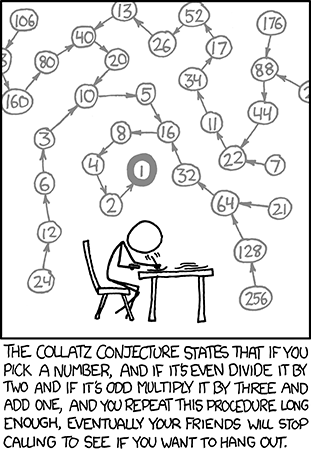
\includegraphics[width=.9\linewidth]{./gfx/08-xkcd-collatz}

\footnotesize
\emph{The Strong Collatz Conjecture states that this holds for any set of obsessively-hand-applied rules."}\\
\url{https://xkcd.com/710/}
\end{columns}
%
\end{frame}

% =========================================================================== %

\begin{frame}[fragile]
%
\begin{columns}[T]
\column{.7\linewidth}
\begin{codebox}[A Collatz Sequence Generator]
\begin{minted}[fontsize=\footnotesize, linenos]{python3}
class Collatz:
    def __init__(self, n):
        self.n = 2 * n

    def __iter__(self):
        return self

    def __next__(self):
        if self.n % 2 == 0:
            self.n = self.n // 2
        else:
            if self.n == 1: raise StopIteration
            self.n = 3 * self.n + 1
        return self.n

for num in Collatz(9):
    print(num)
\end{minted}
\end{codebox}
%
\column{.2\linewidth}
\begin{cmdbox}[Output]
\begin{minted}[fontsize=\footnotesize]{text}
9   13
28  40
14  20
7   10
22  5
11  16
34  8
17  4
52  2
26  1
\end{minted}
\end{cmdbox}
%
\footnotesize
\emph{Read column-wise. Output has been wrapped to fit on this slide.}
\end{columns}
%
\end{frame}

% =========================================================================== %

\begin{frame}{To Put It In A Nutshell ...}
%
\begin{itemize}
\item The Iterable
	\begin{itemize}
	\item Is instance of a (user defined) \inPy{class}
	\item Defines at least a method \inPy{__iter__} which returns an iterator
	\end{itemize}
\item The Iterator
	\begin{itemize}
	\item Is instance of a (user defined) \inPy{class}, too
	\item Can be distinct from or integrated in the iterable
	\item Knows about the iterable if distinct
	\item Defines a method \inPy{__next__}
		\begin{itemize}
		\item Usually updates book keeping variables within the iterator instance
		\item Returns whichever is the next element of the iterable
		\item May change the iterable itself (\Thus \emph{consuming iteration})
		\item \inPy{raise}s \texttt{StopIteration} when last element has been emitted
		\end{itemize}
	\end{itemize}
\item Consuming Iteration
	\begin{itemize}
	\item After Iteration, data cannot be reproduced
	\item Useful, if single use anyway and memory consumption of greater concern
	\item Enables \emph{infinite} sequences, \zB´ all (even) integers, primes, ...
	\end{itemize}
\end{itemize}
%
\end{frame}

% =========================================================================== %

\begin{frame}
%
\begin{hintbox}[Example: Tree Structure]
See GRIPS for a more involved example that shows how to build and store a tree structure (on the example of a file system) and how to iterate over the tree.

\vspace{6pt}
The tree itself is modelled as (something like) nested lists. Note how a single index won't do in this case -- you need to give list indices for each level. So the \enquote{magic} here lies in correctly updating the indices.

\vspace{6pt}
True to the nature of a tree as a \emph{self similar structure}, this example also helps you to refresh your skills in \emph{recursive algorithms}.
The actual iterator, however, is implemented in a non-recursive manner.
\end{hintbox}
%
\end{frame}

% =========================================================================== %

\begin{frame}[fragile]{Cutting Down to the Essential Bits -- the Command \inPy{yield}}
%
\begin{itemize}
\item Can be used in regular functions
\item Like \inPy{return}: leave function and report value to calling site
\item But: resuming the function (as opposed to restarting) at the next call
	\begin{itemize}
	\item Restarting: all variables in the function are reset
	\item Resuming: the previous values of the function and even the line in which we left it are preserved
	\end{itemize}
\item Think of this as implicitly generating a class with \inPy{__iter__} and \inPy{__next__}
\item The function result becomes an iterable
	\begin{itemize}
	\item More precisely: \emph{generator object}
	\item Actually has \inPy{__iter__} and \inPy{__next__}
	\item End of iteration not by \inPy{raise StopIteration}, but simply by exiting the function (\inPy{return None} or going beyond the last code line of the function)
	\end{itemize}
\item Changing internal state of function \Thus consuming iteration
\end{itemize}
%
\end{frame}

% =========================================================================== %

\begin{frame}[fragile]
%
\begin{codebox}[A Generator Function]
\begin{minted}[fontsize=\footnotesize, linenos]{python3}
def collatz(n):
    yield n
    while n != 1:
        if n % 2 == 0: n //= 2
        else:          n = 3 * n + 1
        yield n

for num in collatz(9):
    print(num)
\end{minted}
\end{codebox}
%
Output: \emph{Same as the previous example}
%
\begin{hintbox}[Short-Form for Consumable Iterables]
When implementing a consumable sequence, \inPy{yield} allows to focus on the interesting bits.
\end{hintbox}
%
\end{frame}

% =========================================================================== %

\begin{frame}[fragile]{Double-Concentrated: Generator Comprehension Expressions}
%
\begin{itemize}
\item For particularly simple/regular sequences: short syntax
	\begin{codebox}[]
	\footnotesize
	\inPy{generator = (expression(variable) for variable in iterable)}
	\end{codebox}
\item expands to
\begin{codebox}[]
\begin{minted}[fontsize=\footnotesize, linenos]{python3}
def hidden_function():
    for variable in iterable:
        yield expression(variable)
generator = hidden_function()
\end{minted}
\end{codebox}
\item[\Thus] key characteristics: parenthesis and \inPy{for}
\end{itemize}
%
\end{frame}

% =========================================================================== %

\begin{frame}

\begin{hintbox}[Tuple Comprehensions]
Other than \inPy{list}s and \inPy{dict}s, tuples cannot be generated from comprehensions \emph{directly}. However, you can put any \emph{iterable} into the \inPy{tuple} constructor.\\
Generator comprehensions are iterables.

\vspace{6pt}
\Thus \inPy{tuple(expression(variable) for variable in iterable))}
\end{hintbox}
%
\end{frame}

% =========================================================================== %

\begin{frame}[fragile]{Iterator invalidation}
%
\begin{itemize}
\item Iterator is separate object from iterable
\item[\Thus] Changes to the iterable not always reflected in the iterator
\item[\Thus] During iteration (\ie in a \inPy{for} loop), do not ...
	\begin{itemize}
	\item Remove items
	\item Add items
	\end{itemize}
\item Rather than that, build a new iterable based on the information in the old one
\end{itemize}
%
\begin{hintbox}[Changing Values]
\footnotesize
Due to Python's object model (\inPy{list}s, \inPy{set}s etc. only contain references to the actual object), changing individual values within an iterable are \emph{usually} fine. This needs not hold in general, as the inner structure of an iterable can be literally anything.
\end{hintbox}
%
\end{frame}

% =========================================================================== %

\begin{frame}[fragile]
%
\begin{codebox}[Invalidated Iterators]
\begin{minted}[fontsize=\footnotesize, linenos]{python3}
data = [2, 3, 5, 7, 8, 10, 11]

for i, num in enumerate(data):
    if num % 2 == 0:
        print("removing", num, "at index", i)
        del data[i]

print(data) # [3, 5, 7, 10, 11], but 10 is even!
# better: data = [num for data if num % 2 == 1]

data = {1, 2, 3}
try:
    for num in data:
        if num % 2 == 1:
             data.add(2 * num)
except RuntimeError as e:
    print("Operation failed:", e)   # Operation failed: Set changed size 
                                    # during iteration
\end{minted}
\end{codebox}
%
\end{frame}

% =========================================================================== %

\begin{frame}[fragile]{Paradigm: Functional Programming}
%
\begin{itemize}
\item Observation: humans are bad at tracking dependencies
	\begin{itemize}
	\item What affects variables, output on screen and disk, ...
	\item[\Thus] Evolution of state
	\end{itemize}
\item One solution: \emph{functional programming}
	\begin{itemize}
	\item Everything is a (pure) function: \enquote{no side effects}, \enquote{no state}
	\item Inputs (\ie function arguments) are not changed by function
	\item Outputs go to end-consumer (screen, disk, ...) or are new inputs to other functions
	\end{itemize}
\item Foundational concept of multiple languages
	\begin{itemize}
	\item E.\;g. Haskell, Lisp, OCaml, ...
	\end{itemize}
\item Python
	\begin{itemize}
	\item Allows the paradigm, doesn't force it onto you
	\item Some neat tricks with iterators
	\end{itemize}
\end{itemize}
%
\end{frame}

% =========================================================================== %

\begin{frame}{Paradigm: Lazy Evaluation}
%
\begin{itemize}
\item \emph{Delayed Evaluation} or \emph{Call By Need}
\item Idea: store instructions how to get results rather than results themselves
\item Advantages
	\begin{itemize}
	\item Possibly infinite data structures (\zB \emph{the sequence of even integers})
	\item Saves memory 
		\begin{itemize}
		\item ... which can make computation \emph{more} efficient when memory would be allocated very frequently and evaluating cannot be parallelized well
		\item ... which makes solving some problems possible in the first place (see bonus slides)
		\end{itemize}
	\item Save computation time if not all possible results are needed
		\begin{itemize}
		\item E.\;g.: Give me $f(x)$ for all $x$ in a \inPy{list} where $x$ is a prime.
		\end{itemize}
	\end{itemize}
\item Disadvantages
	\begin{itemize}
	\item Comes at the expense of less efficient computation (or needing black magic in the compiler)
	\item Requires (pure) functional programming approach
	\end{itemize}
\item Mostly, code that reads more nicely, at the expense of \emph{some} time efficiency
\end{itemize}
%
\end{frame}

% =========================================================================== %

\begin{frame}{Example: Non-Functional vs. Functional Approach}
%
\begin{itemize}
\item Give me $f(x)$ for all $x$ in a \inPy{list} where $x$ is a prime.
\item Non-Functional Approach 1: Remove all non-primes from the list, then overwrite the rest with $f(x)$ for each $x$ in the list
	\begin{itemize}
	\item Does no other point in the code need the list elements any longer?
	\item Do we need to update a list-length variable or the like?
	\end{itemize}
\item Non-Functional Approach 2: Copy all primes into a new list, then compute $f(x)$ for each element in the new list
	\begin{itemize}
	\item Possibly a lot of copying
	\item What happens to the new list after we're done with it? Any maintained references?
	\item Do changes in the new list affect the original one?
	\end{itemize}
\item Functional approach
	\begin{itemize}
	\item Construct an iterator that only returns the primes
	\item Compute $f(x)$ for each value the iterator returns
	\item Bonus points: construct an iterator that returns $f(x)$
	\end{itemize}
\end{itemize}
%
\end{frame}

% =========================================================================== %

\begin{frame}[fragile]{Python Goodies: \inPy{filter} and \inPy{map}}
%
\begin{itemize}
\item \inPy{filter}
	\begin{itemize}
	\item Takes a function \texttt{f: x} \thus \inPy{bool}
	\item And an iterable
	\item Returns iterator that only returns the objects where \inPy{f(x) == True}
	\end{itemize}
\item \inPy{map}
	\begin{itemize}
	\item Takes a function \texttt{f: x} \thus \inPy{object}
	\item And an iterable
	\item Returns iterator that returns the objects where \inPy{f(x)} for each \texttt{x} in the iterable
	\end{itemize}
\item[\Thus] \inPy{map(f, filter(is_prime, my_numbers))}
\end{itemize}
%
\begin{hintbox}[List Comprehension Often More Concise]
\footnotesize
For \emph{simple} examples, it is often clearer readable to use the comprehension syntax. The above example can also be realized with:
\mint{python3}{(f(x) for x in my_numbers if is_prime(x))}
\end{hintbox}
%
\end{frame}

% =========================================================================== %

\begin{frame}{Tangent: Short Circuiting}
%
\begin{itemize}
\item Functional thinking sometimes reveals potential for optimization
\item Example: logical operators
	\begin{itemize}
	\item \inPy{expression_1() and expression_2()}
		\begin{itemize}
		\item If \texttt{expression\_1()} is \inPy{False}, there's no need to evaluate \texttt{expression\_2()}
		\end{itemize}
	\item \inPy{expression_1() or expression_2()}
		\begin{itemize}
		\item If \texttt{expression\_1()} is \inPy{True}, there's no need to evaluate \texttt{expression\_2()}
		\end{itemize}
	\end{itemize}
\item[\Thus] Save time by only evaluating \texttt{expression\_2()} if it can change the result of the logical conjunction
\item[\Thus] Python does this automatically
\item[\Thus] Implicit assumption: No side effects!
\end{itemize}
%
\end{frame}

% =========================================================================== %

\begin{frame}[fragile]
%
\begin{codebox}[Short Circuiting]
\begin{minted}[fontsize=\footnotesize, linenos]{python3}
import time

def say_A: print("A"); return True
def say_B: print("B"); return True

if say_A() or say_B(): pass    # only prints A

a, b = say_A(), say_B()        # prints A and B
if a or b: pass

def quick_to_evaluate: return False
def slow_to_evaluate: time.sleep(2); return False

if slow_to_evaluate() and quick_to_evaluate(): pass   # takes 2 seconds
else: print("Wasted time by failing to leverage short circuiting")

if quick_to_evaluate() and slow_to_evaluate(): pass   # takes almost no time
else: print("Got the same result way faster")
\end{minted}
\end{codebox}
%
\end{frame}

% =========================================================================== %

\begin{frame}{The Module \texttt{itertools}}
%
\begin{itemize}
\item Dedicated module to produce very useful iterators
\item General purpose and combinatoric functions
\item See \url{https://docs.python.org/3/library/itertools.html}
\item Some of them seem to do the same as other existing functions/concepts, but there always are subtle differences
\item Takes some time to get used to them, but ...
\item ... if you know what the module provides, you get stuff done much faster
\end{itemize}
%
\begin{hintbox}[Like Lego Bricks]
\small
The strength in the itertools module is that all its functions work together. The output of one function can be used as input for another function.
\end{hintbox}
%
\end{frame}

% =========================================================================== %

\begin{frame}{Infinite Iterators: \texttt{count}, \texttt{cycle} and \texttt{repeat}}
%
\begin{itemize}
\item \texttt{count}: like \inPy{range}, but no end point.\\
	Literally like \inPy{range(start, step, infinity)}
	\begin{itemize}
	\item E.\;g.: \inPy{itertools.count(5)} \thus \texttt{5, 6, 7, 8, 9, ...}
	\item E.\;g.: \inPy{itertools.count(5, 2)} \thus \texttt{5, 7, 9, 11, ...}
	\end{itemize}
\item \texttt{cycle}: repeat the same sequence over and over again
	\begin{itemize}
	\item E.\;g.: \inPy{itertools.cycle("abc")} \thus \texttt{a, b, c, a, b, ...}
	\end{itemize}
\item \texttt{repeat}: repeats a single element endlessly or up to \texttt{n} times
	\begin{itemize}
	\item E.\;g.: \inPy{itertools.repeat("abc")} \thus \texttt{abc, abc, abc, ...}
	\item E.\;g.: \inPy{itertools.repeat("abc", 3)} \thus \texttt{abc, abc, abc}
	\end{itemize}
\end{itemize}
%
\end{frame}

% =========================================================================== %

\begin{frame}[fragile]{Cousins to \inPy{filter} and \inPy{map}}
%
\begin{itemize}
\item \texttt{starmap}: Like \inPy{map}, but supports functions with more than one argument
	\begin{itemize}
	\item Calls \inPy{f(*next(iterator))} -- hence the name \emph{star}map
	\item Implicit assumption: elements of iterable are iterables themselves
	\item Example:
		\begin{itemize}
		\item \inPy{get_length = lambda x, y: math.sqrt(x*x + y*y)}
		\item \inPy{vectors = [(1, 2), (5, 2), ...]}
		\item \inPy{vector_lengths = itertools.starmap(get_length, vectors)}
		\end{itemize}
	\end{itemize}
\item \texttt{filterfalse}: like \inPy{filter}, but only retains those where \texttt{f(x)} is \inPy{False}
\item \texttt{dropwhile} and \texttt{takewhile}
	\begin{itemize}
	\item Similar to \inPy{filter}, but only accept/remove items until the first \inPy{False}
	\item E.\;g.: \inPy{takewhile(lambda x: x<5, [1,4,6,4,1])} \thus \texttt{1, 4}
	\end{itemize}
\end{itemize}
%
\begin{hintbox}[First Synergy]
\footnotesize
\texttt{dropwhile} and \texttt{takewhile} work very well with the infinite iterators from the previous slide.
\end{hintbox}
%
\end{frame}

% =========================================================================== %

\begin{frame}{(Partial) Reductions}
%
\begin{itemize}
\item Reduction: \emph{collection of elements} \thus \emph{single element}
\item Example: \inPy{sum}
\item \texttt{itertools.accumulate}: \emph{partial} reduction
	\begin{itemize}
	\item \emph{collection of elements} \thus \emph{collection of elements}
	\item Idea: \inPy{result[i] = sum(input_iterable[:i+1])}\\
		\emph{(Note: this syntax works only for indexable iterables like \inPy{list}s. \texttt{accumulate} works for any iterable.)}
	\end{itemize}
\item \texttt{functools.reduce}: arbitrary reduction
	\begin{itemize}
	\item Takes three parameters: reducing function, iterable and initial value
	\item Reducing function: two parameters: \texttt{accumulator} and \texttt{next\_value}
	\item Returns updated \texttt{accumulator}
	\item E.\;g.: \inPy{array_product = lambda acc, nxt: acc * nxt}
	\item \inPy{twenty_four = functools.reduce(array_product, [1, 2, 3, 4], 1)}
	\end{itemize}
\end{itemize}
%
\end{frame}

% =========================================================================== %

\begin{frame}[fragile]{Combinatorics}
%
\begin{itemize}
\item \texttt{product}: Outer product of iterables, aka all possible combinations of their elements
	\begin{itemize}
	\item Produces \inPy{tuple}s of the combined items
	\item Essentially: nexted loops, or \texttt{np.meshgrid}
	\item E.\;g.: \inPy{itertools.product([1, 2], "ab")} \thus \inPy{(1, 'a'), (1, 'b'), (2, 'a'), (2, 'b')}
	\end{itemize}
\item \texttt{permutations}: All \texttt{tuple}s (of given length) that can be formed from the original elements
	\begin{itemize}
	\item \inPy{itertools.permutations("abc")} \thus \texttt{abc, acb, bac, bca, cab, cba}
	\item \inPy{itertools.permutations("abc", 2)} \thus \texttt{ab, ac, ba, bc, ca, cb}
	\end{itemize}
\item \texttt{combinations}: All \texttt{tuple}s of given length \emph{without repeated elements}
	\begin{itemize}
	\item \inPy{itertools.combinations("abc", 2)} \thus \texttt{ab, ac, bc}
	\end{itemize}
\item \texttt{combinations\_with\_replacements}: likewise, but allows \texttt{tuple}s with same element twice
	\begin{itemize}
	\item \inPy{itertools.combinations_with_replacements("abc", 2)} \thus \texttt{aa, ab, ac, bb, bc, cc}
	\end{itemize}
\end{itemize}
%
\end{frame}

% =========================================================================== %

% https://realpython.com/python-filter-function/
% https://realpython.com/python-reduce-function/

% =========================================================================== %

\begin{frame}{Bonus: Sweets Budget}
%
\begin{itemize}
\item Example Problem: Optimization of Sweets Buying Strategy
	\begin{itemize}
	\item Limited budget, different sweets with different prices and rating
	\item[\Thus] Buy combination with highest rating that is still within budget
	\end{itemize}
\item Brute Force Approach
	\begin{itemize}
	\item Find all possible combinations
	\item Filter out those which are out of budget
	\item Compute ratings of all combinations
	\item Find best one
	\end{itemize}
\item Implementation with numpy (eager evaluation) and itertools (lazy evaluation)
\end{itemize}
%
\end{frame}

% =========================================================================== %

\begin{frame}[fragile]
%
\begin{codebox}[Sweets Numpy ...]
\begin{minted}[fontsize=\footnotesize, linenos]{python3}
money = 10.0
names = ["dark chocolate", "milk chocolate", "caramel nuts bar", 
         "coco cubes", "mint drops"]
prices = np.array([1.0, 0.9, 2.3, 1.5, 0.3])
weights = np.array([5, 4, 12, 8, 1])

upper_limits = money // prices
values = tuple([np.arange(u + 1) for u in upper_limits])
meshgrid = np.meshgrid(*values)

total_money = np.zeros(meshgrid[0].shape)
for i, price in enumerate(prices):
    total_money += price * meshgrid[i]

totalScore = np.zeros(meshgrid[0].shape)
for i, score in enumerate(weights):
    totalScore += score * meshgrid[i]
\end{minted}
\end{codebox}
%
\end{frame}

% =========================================================================== %

\begin{frame}[fragile]
%
\begin{codebox}[... Continued]
\begin{minted}[fontsize=\footnotesize, linenos, firstnumber=last]{python3}
mask = total_money > money
totalScore[mask] = -1

best_id = np.argmax(totalScore)
bestConfig = np.unravel_index(best_id, shape=meshgrid[0].shape)
\end{minted}
\end{codebox}
%
\end{frame}

% =========================================================================== %

\begin{frame}[fragile]
%
\begin{codebox}[Sweets Lazy Evaluation ...]
\begin{minted}[fontsize=\footnotesize, linenos]{python3}
money = 10.0
sweets_price_and_score = {
    "dark chocolate": (1.0, 5),
    "milk chocolate": (0.9, 4),
    "caramel nuts bar": (2.3, 12),
    "coco cubes": (1.5, 8),
    "mint drops": (0.3, 1),
}

upper_limits = map(lambda price_and_score: int(money // price_and_score[0]), 
                   sweets_price_and_score.values())

individual_counts = (range(0, u + 1) for u in upper_limits)

configurations = itertools.product(*individual_counts)
\end{minted}
\end{codebox}
%
\end{frame}

% =========================================================================== %

\begin{frame}[fragile]
%
\begin{codebox}[... Continued]
\begin{minted}[fontsize=\footnotesize, linenos, firstnumber=last]{python3}
get_price_for_configuration = lambda config: (sum(qty * evaluation[0] 
    for qty, evaluation 
    in zip(config, sweets_price_and_score.values())), config)
prices = map(get_price_for_configuration, configurations)

get_value_for_configuration = lambda price, config: (sum(qty * evaluation[1]
    for qty, evaluation in zip(config, sweets_price_and_score.values())),
    price, config)
values_affordable = itertools.starmap(
    get_value_for_configuration, 
    filter(lambda price: price[0] <= money, prices)
)

best_value, best_price, best_config = max(
    values_affordable, 
    key=lambda all_data: all_data[0]
)
\end{minted}
\end{codebox}
%
\end{frame}

% =========================================================================== %

\begin{frame}{Results in Comparison}
%
\begin{center}
\rowcolors{1}{white}{tabhighlight}
\begin{tabular}{cc|rr}
	\textbf{Implementation} & \textbf{Sweets} & \textbf{Runtime} & \textbf{Memory Footprint} \\ \hline %tabcrlf
	Eager (Numpy)           &              5  &             4 ms &   2.55 MB \\
	Eager (Numpy)           &              6  &            82 ms &  28 MB \\
	Eager (Numpy)           &              7  &           729 ms & 168 MB \\
	Eager (Numpy)           &              8  & (did not finish) & more than 2 GB \\ 
\hline
	Lazy (Iterators)        &              5  &           112 ms & 352 Bytes \\
	Lazy (Iterators)        &              6  &         1 334 ms & 360 Bytes \\
	Lazy (Iterators)        &              7  &         8 329 ms & 368 Bytes \\
	Lazy (Iterators)        &              8  &        39 529 ms & 376 Bytes 
\end{tabular}
\end{center}
%
\begin{hintbox}[Confucius says]
Finishing slowly beats failing fast.
\end{hintbox}
%
\end{frame}

% =========================================================================== %